\section{Alit Fajar Kurniawan 1174057}

\subsection{Teori}
\begin{enumerate}
\item Jelaskan apa itu klasifikasi teks, sertakan gambar ilustrasi buatan sendiri.
\par Klasifikasi teks adalah proses pemberian tag atau kategori ke teks sesuai dengan isinya. Teks dapat menjadi sumber informasi yang sangat kaya, tetapi mengekstraksi wawasan darinya bisa sulit dan memakan waktu karena sifatnya yang tidak terstruktur. berikut contoh gambar \ref{klasifikasi teks} .
\begin{figure}[H]
\centering
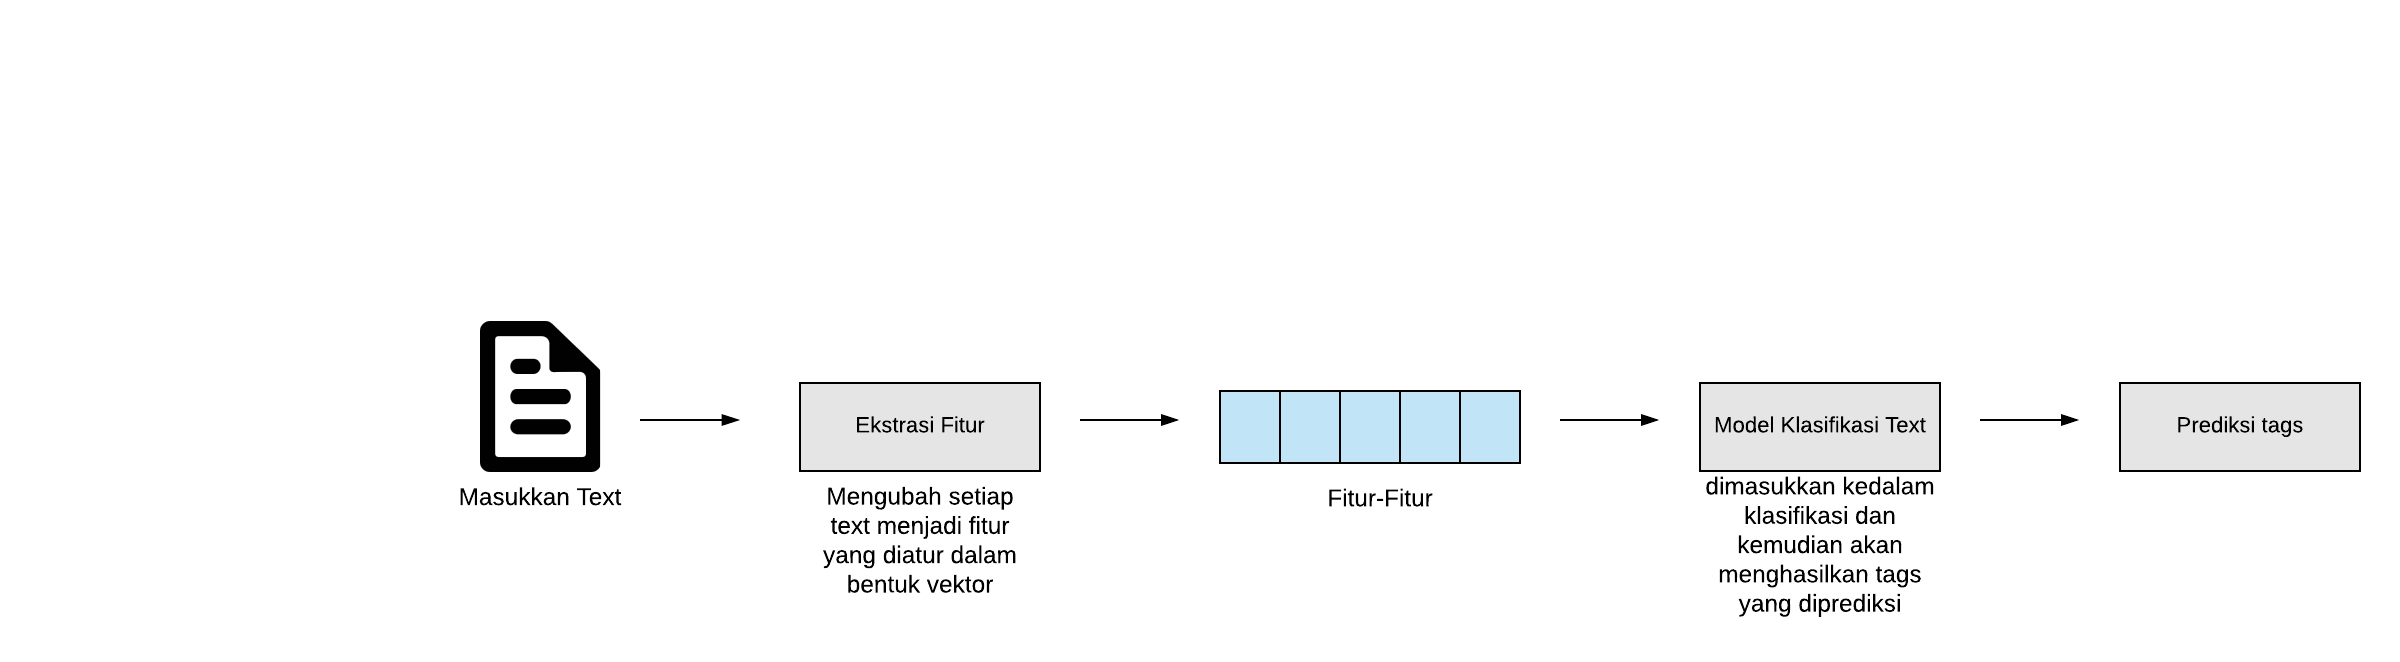
\includegraphics[scale=0.2]{figures/1174057/chapter4/1.png}
\caption{contoh klasifikasi teks}
\label{klasifikasi teks}
\end{figure}

\item Jelaskan mengapa klasifikasi bunga tidak bisa menggunakan machine learning, sertakan ilustrasi sendiri.
\par Untuk klasifikasi bunga tidak dapat menggunakan machine learning dikarenakan memiliki masalah input yang sama namun keluarannya (output) yang berbeda, biasanya output atau error ini disebut dengan istilah ’noise’. Noise sendiri merupakan output yang disimpan / ditangkap maupun direkam bukan seperti seharusnya ( keluaran yang diiginkan ). Apabila diberikan contoh, maka contohnya yaitu kita berasumsi secara implisit bahwa klarifikasi bunga yang kita lakukan sudah tepat dan kita melakukannya seperti seorang ahli tanaman. Namun pada hasilnya masih saja terjadi kesalahan. Selain itu, selalu ada peluang untuk memperkenalkan kesalahan saat merekam ataupun menyimpan data, maka harus dilakukan penelitian yang lebih rinci sehingga tidak menimbulkan ’noise’ itu sendiri. Berikut ilustrasi gambar \ref{gambar bunga}
\begin{figure}[H]
\centering
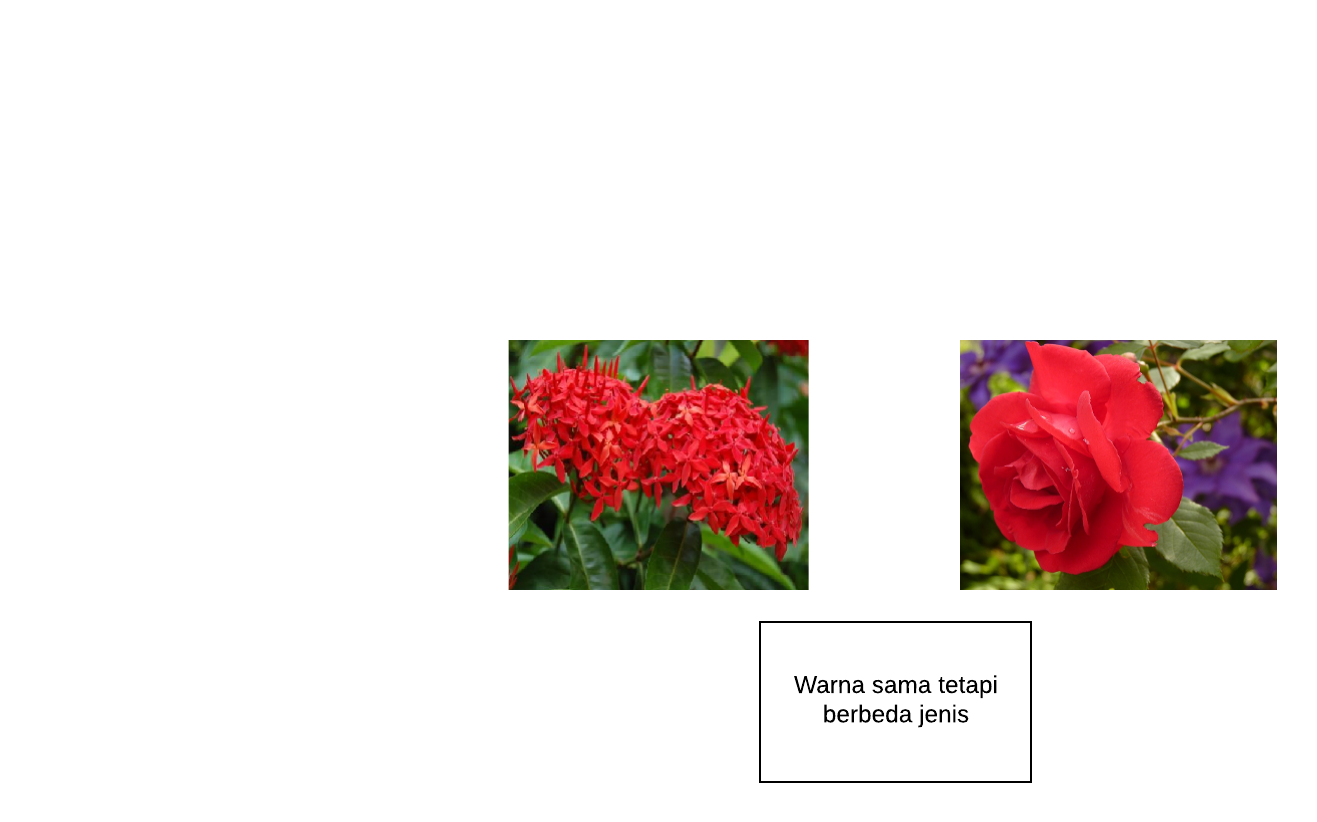
\includegraphics[scale=0.3]{figures/1174057/chapter4/2.png}
\caption{gambar bunga}
\label{gambar bunga}
\end{figure}

\item Jelaskan bagaimana teknik pembelajaran mesin pada teks pada kata-kata yang digunakan di youtube,jelaskan arti per atribut data csv dan sertakan ilustrasi buatan sendiri.
\par Kita ambil sebuah kasus yang semua orang telah ketahui dan juga pahami. Kasus tersebut yaitu perekomendasian video dari pencarian menggunakan ”text / kata” di Youtube. Pada saat menggunakan Youtube terdapat Machine Learning yang bekerja dan memproses perintah ataupun aktivitas tersebut, dimana akan memfilter secara otomatis video yang disesuaikan dengan ”keyword” yang kita masukkan sehingga memberikan keluaran video dengan keyword yang benar. Adapula fitur yang di dapatkan ketika sedang menonton Youtube. Tampilan sebelah kanan terdapat pilihan ’Next’ atapun ’Suggestion’ yang menampilkan beberapa video serupa sesuai dengan yang dicari atau sedang ditonton. Ketika mengklik salah satu video dari baris tersebut, maka Youtube akan mengingat dan menggunakan kata yang tertera sebagai referensi kembali sehingga akan memberikan kemudahan pada pencarian yang lainnya, Dan disitulah mesin belajar sendiri dan menyimpan data secara berkala sehingga berkembang. contoh pada gambar \ref{pembelajaran mesin}
\begin{figure}[H]
\centering
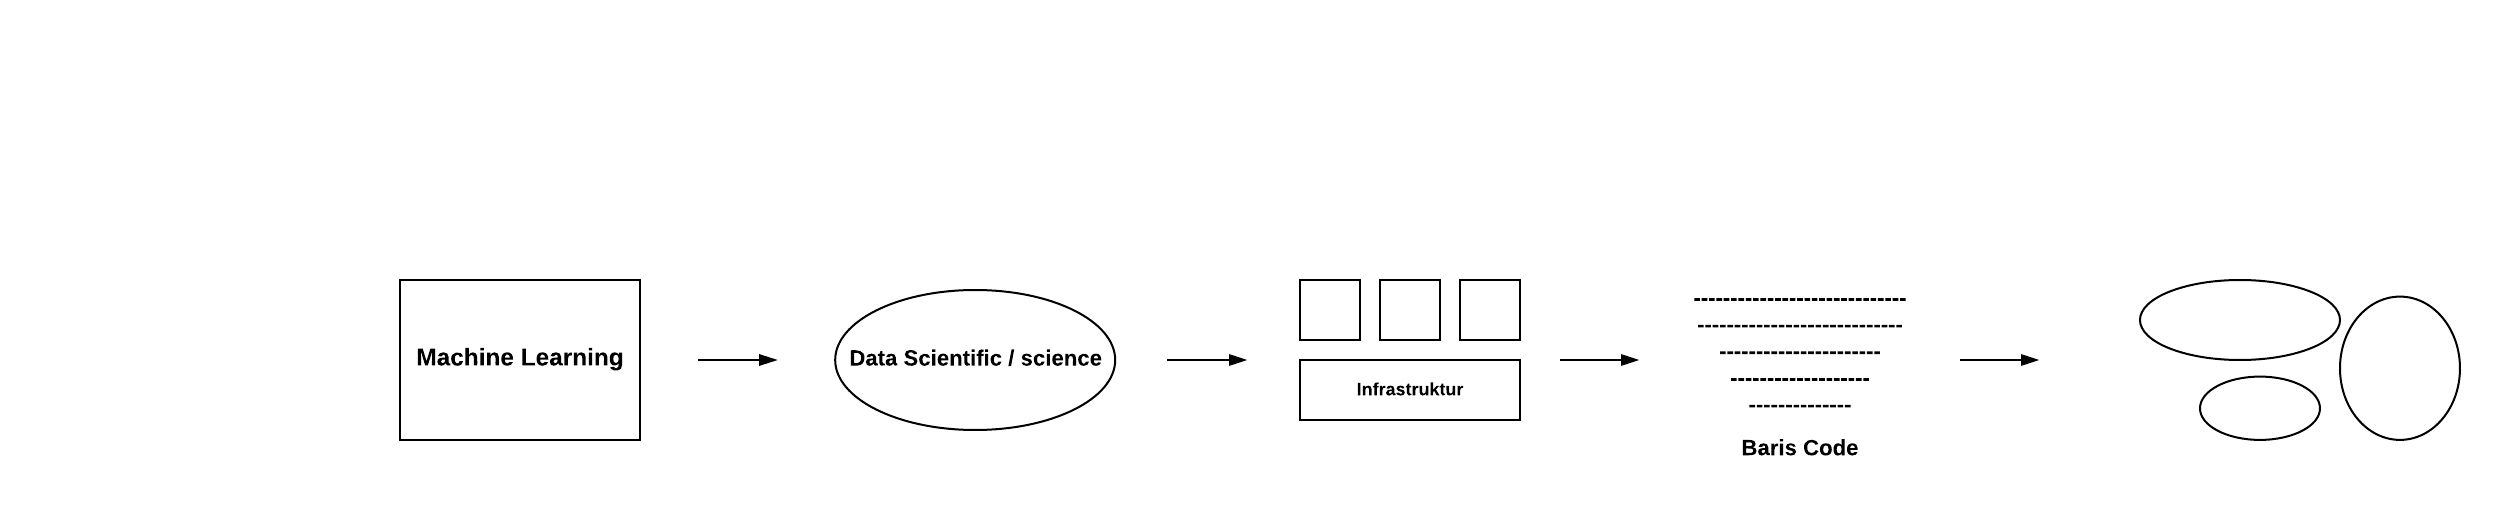
\includegraphics[scale=0.2]{figures/1174057/chapter4/3.png}
\caption{pembelajaran mesin}
\label{pembelajaran mesin}
\end{figure}

\item Jelaskan apa yang dimaksud vektorisasi data.
\par Pembagian dan pemecahan data, kemudian dilakukan perhitungan. Vektorisasi juga dapat dimaksudkan dengan setiap data yang mungkin dipetakan ke integer tertentu. jika kita memiliki array yang cukup besar maka setiap kata / data cocok dengan slot unik dalam array (nilai pada indeks adalah nomor satu kali kata itu muncul).
\par Array angka floating point ( Mewakili data ) :
\begin{itemize}
\item teks
\item audio
\item gambar
\end{itemize}
\par Contoh : -[1.0, 0.0, 1.0, 0.5]

\item Jelaskan apa itu bag of words dengan kata-kata yang sederhana dan ilustrasi sendiri.
\par bag-of-words adalah representasi penyederhanaan yang digunakan dalam pemrosesan bahasa alami dan pengambilan informasi. Model bag-of-words sederhana untuk dipahami dan diterapkan dan telah melihat kesuksesan besar dalam masalah seperti pemodelan bahasa dan klasifikasi dokumen.Pada model ini, tiap kalimat dalam dokumen digambarkan sebagai token, mengabaikan tata bahasa dan bahkan urutan kata namun menghitung frekuensi kejadian atau kemunculan kata dari dokumen. berikut contoh gambar \ref{bag of words}
\begin{figure}[H]
\centering
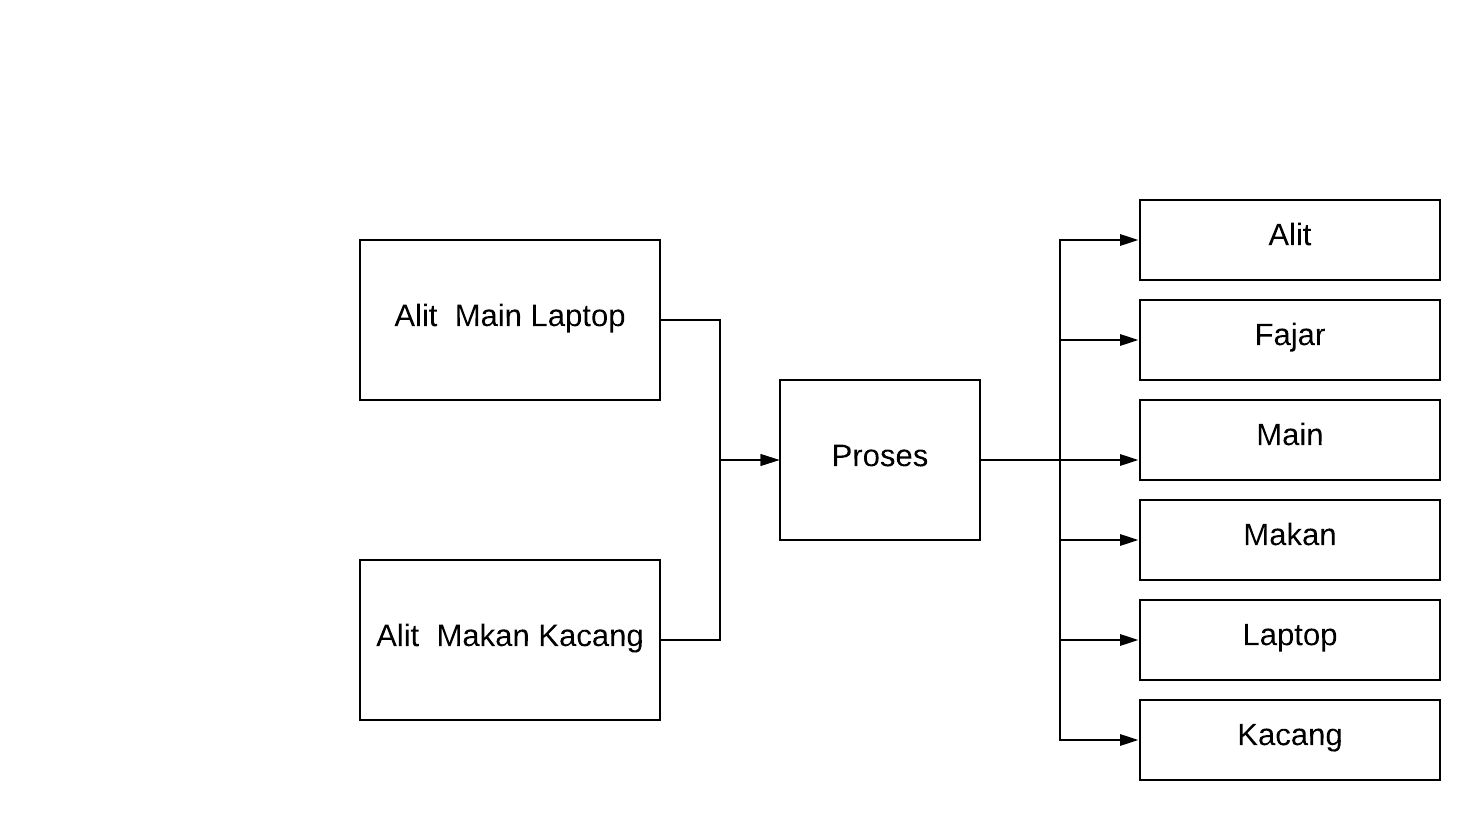
\includegraphics[scale=0.5]{figures/1174057/chapter4/4.png}
\caption{bag of words}
\label{bag of words}
\end{figure}

\item Jelaskan apa itu TF-IDF, ilustrasikan dengan gambar sendiri
\par TF-IDF memberi kita frekuensi kata dalam setiap dokumen dalam korpus atau mengganti data jadi number. Ini adalah rasio berapa kali kata itu muncul dalam dokumen dibandingkan dengan jumlah total kata dalam dokumen itu. Itu meningkat seiring jumlah kemunculan kata itu di dalam dokumen meningkat. Setiap dokumen memiliki tf sendiri.
\begin{figure}[H]
\centering
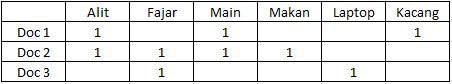
\includegraphics[scale=0.6]{figures/1174057/chapter4/5.PNG}
\caption{TF-IDF}
\label{TF-IDF}
\end{figure}

\end{enumerate}

\subsection{Praktek Program}
\begin{enumerate}
\item import data pandas dan 500 baris data dummy kemudian di jelaskan tiap barisnya.
\lstinputlisting[firstline=8, lastline=18]{src/1174057/chapter4/1174057.py}
\begin{figure}[H]
\centering
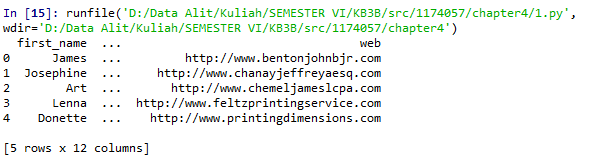
\includegraphics[scale=0.7]{figures/1174057/chapter4/6.PNG}
\caption{hasil}
\label{Praktek no 1}
\end{figure}		

\item dari dataframe tersebut dipecah menjadi dua dataframe yaitu 450 row pertama dan 50 row sisanya
\lstinputlisting[firstline=19, lastline=23]{src/1174057/chapter4/1174057.py}
\begin{figure}[H]
\centering
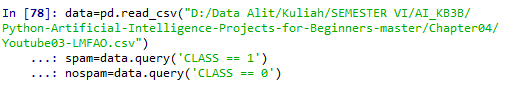
\includegraphics[scale=0.7]{figures/1174057/chapter4/7_1.PNG}
\caption{hasil}
\label{Praktek}
\end{figure}

\begin{figure}[H]
\centering
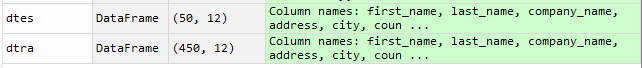
\includegraphics[scale=0.7]{figures/1174057/chapter4/7.PNG}
\caption{hasil}
\label{Praktek no 2}
\end{figure}		

\item praktek vektorisasi
\lstinputlisting[firstline=28, lastline=58]{src/1174057/chapter4/1174057.py}	
\par lakukan import library pandas yang di inisialisasi menjasi pd setelah itu ada dibuat variable data dengan method read\_csv untuk membaca file berekstensikan csv yang di masukan alamatnya pada kurung, lakukan klasifikasi atau pemilihan komentar yang berisi spam atau bukan spam dengan parameter class samadengan 1 merupakan spam dan class samadengan 0 bukan spam setelah itu masukan librari CountVektorizer yang digunakan untuk vektorisasi data kemudian dilanjutkan pada bagian In[103] dibuat variabel yang berisi vektorisasi dari data pada data di field content setelah itu variabel tersebut di running hasilnya menunjukan 350 baris di kali 1738 kolom selanjutnya dicoba untuk memunculkan isi recod pada baris ke 345 maka akan muncul isian dari baris tersebut. selanjutnya dibuat variabel dk atau daftar yang berisi data hasil vektorisasi setelah yang terdiri dari variabel dshuf yang berisi data komen yang di dalamnya di buat random yang nantinya akan dibut data training dan data testing dengan ketentuan data training 300 dan data testing sebanyak 50 setelah itu data training di lakukan vektorisasi dan data testing juga dilakukan vektorisasi setelah itu kedua data training dan testing tersebut dibuat label dengan parameter field CLASS pada tabel.
\begin{figure}[H]
\centering
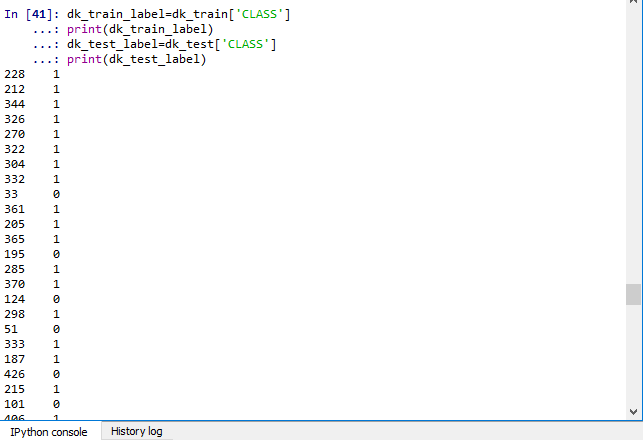
\includegraphics[scale=0.7]{figures/1174057/chapter4/8.PNG}
\caption{hasil}
\label{Praktek no 3}
\end{figure}		

\item klasifikasi SVM
\lstinputlisting[firstline=61, lastline=67]{src/1174057/chapter4/1174057.py}
\begin{figure}[H]
\centering
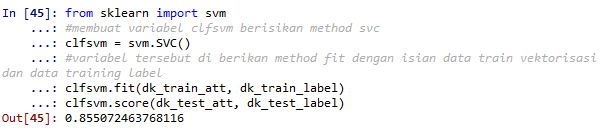
\includegraphics[scale=0.7]{figures/1174057/chapter4/9.PNG}
\caption{hasil}
\label{Praktek no 4}
\end{figure}		

\item klasifikasi decision tree
\lstinputlisting[firstline=70, lastline=74]{src/1174057/chapter4/1174057.py}
\par import librari tree dari sklearn kemudian membuat variabel clftree berisikan method DecisionTreeClasifier setelah itu variabel tersebut di berikan method fit dengan isian data train vektorisasi dan data training label yang berguna untuk melatih data tersebut agar dapat digunakan pada codingan selanjutnya setelah itu di coba untuk memunculkan score atau akurasi dari data tersebut menggunakan data testing vektorisasi dan data testing label.
\begin{figure}[H]
\centering
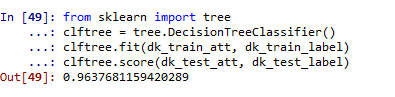
\includegraphics[scale=0.7]{figures/1174057/chapter4/10.PNG}
\caption{hasil}
\label{Praktek no 5}
\end{figure}	

\item plot confusion matrix
\lstinputlisting[firstline=76, lastline=80]{src/1174057/chapter4/1174057.py}
\par import library comfusion matrix selanjutnya dilakukan prediksi pada pada data tes nya kemudian data tersebut di masukan kedalam variabel cm dengan method confusion matrix yang di dalamnya terdapat data dari variabel perd label dan dk test label setelah itu variabel cm tersebut di running maka akan memunculkan nilai matrixnya. 	
\begin{figure}[H]
\centering
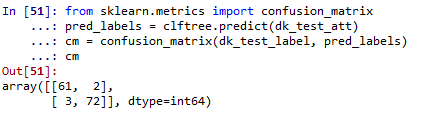
\includegraphics[scale=0.7]{figures/1174057/chapter4/11.PNG}
\caption{hasil}
\label{Praktek no 6}
\end{figure}

\item cross valodation
\lstinputlisting[firstline=83, lastline=101]{src/1174057/chapter4/1174057.py}
\par memunculkan nilai akurasi dari tiga metode yaitu random forest, decision tree, dan klasifikasi svm (suport vector machine) diamana akan di bandingkan tingkat akurasi dari semua hasil akurasiya mana yang terbaik dan lebih akurat pada hasilnya data yang paling akurat yaitu random forest.
\begin{figure}[H]
\centering
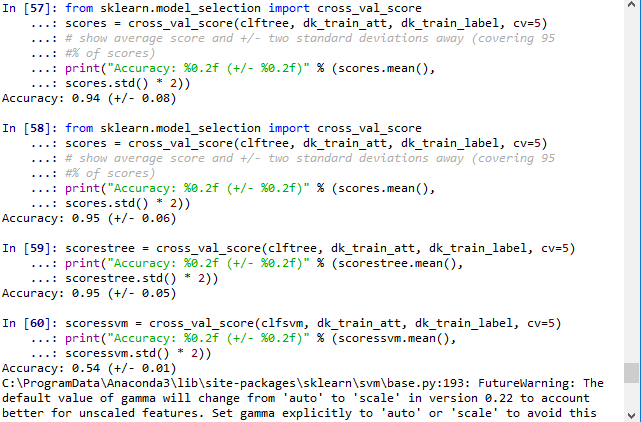
\includegraphics[scale=0.7]{figures/1174057/chapter4/12.PNG}
\caption{hasil}
\label{Praktek no 7}
\end{figure}

\item Pengamatan program
\lstinputlisting[firstline=104, lastline=120]{src/1174057/chapter4/1174057.py}
\par terdapat grafik data yang terdapat dari grafik tersebut di dapat dari codingan dengan cara pengulangan data masing masing 10 kali setelah itu di eksekusi menjadi grafik berbentuk 3D pada gambar tersebut menunjukan rasio dari yang terrendah yaitu data SVM kemudian data decision tree dan hasil random forest.
\begin{figure}[H]
\centering
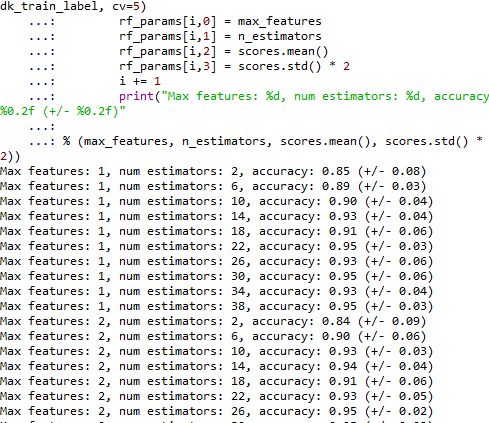
\includegraphics[scale=0.7]{figures/1174057/chapter4/13.PNG}
\caption{hasil}
\label{Praktek no 8}
\end{figure}

\par Berikut adalah untuk grafik
\lstinputlisting[firstline=122, lastline=136]{src/1174057/chapter4/1174057.py}
\begin{figure}[H]
\centering
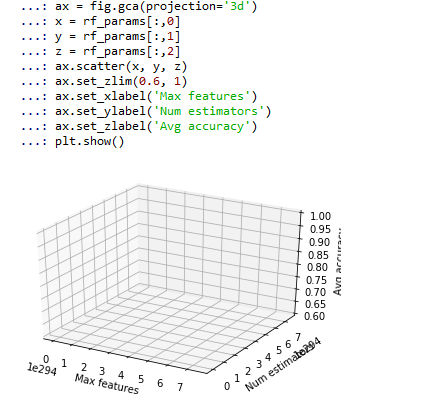
\includegraphics[scale=0.7]{figures/1174057/chapter4/14.PNG}
\caption{hasil}
\label{Praktek no 8 Grafik}
\end{figure}
\end{enumerate}

\subsection{Penanganan Error}
\subsubsection{Sreenshoot Error}
\begin{enumerate}
\item Error 1
\begin{figure}[H]
\centering
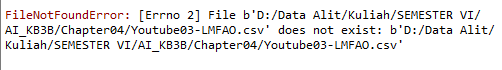
\includegraphics[scale=1]{figures/1174057/chapter4/error1.PNG}
\caption{error 1}
\label{error 1}
\end{figure}        

\item Error 2
\begin{figure}[H]
\centering
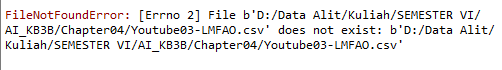
\includegraphics[scale=1]{figures/1174057/chapter4/error1.PNG}
\caption{error 1}
\label{error 1}
\end{figure}       
\end{enumerate} 

\subsubsection{Penanganan Error}
\begin{enumerate}
\item penanganan 1, kesalahan pada alamat direktori yang dituju, jadi harus dipastikan alamat direktori yang benar
\begin{figure}[H]
\centering
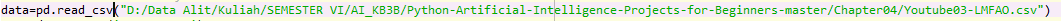
\includegraphics[scale=1]{figures/1174057/chapter4/penanganan1.PNG}
\caption{penanganan1}
\label{penanganan1}
\end{figure}    

\item penanganan 2, RandomForestClassifier belum diimport, sehingga melakukan import library terlebih dahulu agar program jalan
\begin{figure}[H]
\centering
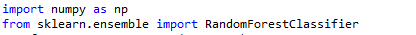
\includegraphics[scale=1]{figures/1174057/chapter4/penanganan2.PNG}
\caption{penanganan2}
\label{penanganan2}
\end{figure}    
\end{enumerate}




